% /Users/pikachu/books/payments-book/src/parts/part4/ch24-decline-management.tex
\chapter{Управление отказами}
\label{ch:decline-management}
\margintoc

\begin{kaobox}[title=Что вы узнаете из этой главы]
  Каждый отказ авторизации выглядит как потерянная выручка, но для
  платёжной системы это прежде всего сигнал: остановиться, повторить
  попытку позже или сменить канал. В этой главе мы разберём, чем мягкий
  отказ (soft decline) отличается от жёсткого, почему код ответа
  \rc{05} нельзя читать буквально, как строить повторы в пределах правил
  \scheme{Visa} и \scheme{Mastercard}, чем сетевой токен помогает
  эмитенту и как маршрутизация через эквайера влияет на долю одобрений.
\end{kaobox}

Когда покупатель видит отказ на странице оплаты, для него всё выглядит
просто: платёж не прошёл. Для платёжной команды на этом простота
заканчивается. Один отказ означает \enquote{подожди и попробуй ещё раз},
другой --- \enquote{эта карта больше не годится}, третий --- \enquote{сломался
маршрут, а не счёт клиента}. Управление отказами и состоит в том, чтобы
различать эти случаи до того, как система начнёт бессмысленно жечь
попытки и раздражать держателя карты.

\section{Анатомия отказа}
\label{sec:decline-anatomy}

На кассе, в приложении и в дашборде все отказы выглядят одинаково:
операция не состоялась. Для системы это не один и тот же тип события.
Если перепутать причину отказа, она либо потратит попытки впустую, либо
нарушит правила схем.

Мягкий отказ (soft decline)\sidenote{Мягкий отказ --- это отказ, который
  может исчезнуть без смены карты или товара: временный лимит,
  поведенческий фильтр, недоступность сервиса или иная обратимая
  причина.} означает, что транзакция отклонена по
временно́й или устранимой причине. Эмитент как будто говорит:
\enquote{не сейчас, попробуй ещё позже}. К мягким отказам обычно относят
\rc{51} --- Insufficient Funds, \rc{05} --- Do Not Honor в ряде контекстов,
\rc{61} --- Exceeds Withdrawal Amount Limit, \rc{62} --- Restricted Card
и \rc{65} --- Exceeds Withdrawal Frequency Limit. Повторная попытка через
некоторое время или через другой канал здесь имеет ненулевые шансы на успех.

Зеркальная ситуация --- жёсткий отказ (hard decline): транзакция отклонена
по постоянной причине, и повтор с теми же реквизитами бессмыслен. К этой
группе относятся \rc{04} --- Pick Up, \rc{14} --- Invalid Account Number,
\rc{41} --- Lost Card, \rc{43} --- Stolen Card и \rc{54} --- Expired Card.
Автоматически повторять такие запросы значит лишь нагружать сети и
раздражать клиента, которому нужна другая карта.

Между этими полюсами есть технические и пограничные коды, где действие
зависит от канала и момента. \rc{01} --- Refer to Card Issuer обычно
требует ручной верификации или иного канала связи с банком. \rc{91} ---
Issuer Unavailable и \rc{96} --- System Malfunction описывают технический
сбой на стороне эмитента или маршрута. Для них уместен один немедленный
повтор, а затем --- пауза и разбор причины~\sidecite{visa-core-rules}\sidecite{mc-rules}.

\begin{figure}
  \centering
  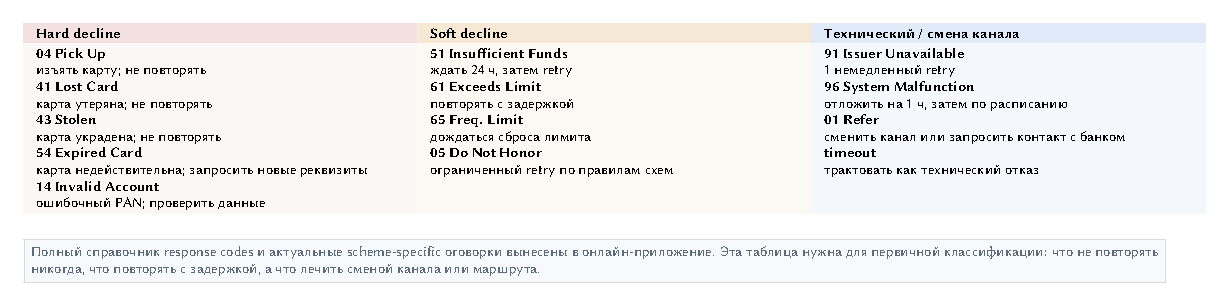
\includegraphics[width=\linewidth]{assets/figures/ch24-decline-management/decline-codes.pdf}
  \caption{Классификация кодов ответа по типу отказа.}
  \label{fig:decline-codes}
\end{figure}

Вывод из этой схемы простой: сначала нужно определить обратимость
отказа, и только потом решать, стоит ли повторять попытку. Код ответа
здесь работает не как диагноз, а как сжатая операционная подсказка.

\section{Что на самом деле означают коды ответа}
\label{sec:decline-response-codes}

У платёжной команды всегда есть соблазн прочитать код ответа как
точную причину отказа. Почти всегда это ошибка. Код ответа
(response code) --- это ответ эмитента, но не его объяснение. За одним
и тем же кодом могут стоять десятки причин, и без дополнительных
данных истинную причину обычно не узнать.

\rc{05} Do Not Honor --- самый распространённый и самый неинформативный
код. Формально он означает \enquote{не проводите операцию}, но почти ничего не
объясняет. За ним могут скрываться антифрод, дневной лимит, несоответствие
поведенческому профилю клиента, временная блокировка в приложении или
внутренняя политика эмитента по конкретному MCC. Часть этих причин
временная и может исчезнуть сама, часть --- постоянная; именно поэтому
\rc{05} обычно трактуют как мягкий отказ, но с осторожным числом повторов.
\scheme{Visa} прямо предупреждает, что часть кодов, сформированных в
режиме stand-in, и часть кодов самого эмитента могут сходиться в
\rc{05}, а \scheme{Mastercard} отдельно контролирует долю этого кода в
CNP-отказах \sidecite{visa-core-rules}\sidecite{mc-rules}.

\rc{51} Insufficient Funds тоже не сводится к буквальному бытовому
смыслу. Для дебетовых карт он действительно часто означает нехватку
средств на счёте. Для кредитных карт это может быть превышение лимита,
а для некоторых эмитентов --- просто универсальная форма мягкого
отказа, когда они не хотят раскрывать более точную причину.

\rc{54} Expired Card встречается чаще, чем следовало бы. Карта может быть
перевыпущена с новой датой истечения, но если Account Updater
(VAU/ABU) ещё не обновил реквизиты у мерчанта, мерчант продолжает
отправлять старую дату \sidecite{visa-core-rules}. Иногда эмитент
возвращает \rc{54} и тогда, когда карта заблокирована в приложении:
формально срок не истёк, но код выбран как эквивалент недействительной карты.

\rc{91} и \rc{96} --- технические коды, которые не говорят о состоянии
карты или счёта. Они означают, что эмитент или маршрут недоступны, а
значит транзакцию уместно повторить, обычно один раз и после короткой
паузы. Если такие
коды доминируют в статистике, проблема часто лежит в сети,
маршрутизации или доступности хоста. Карта здесь может быть вообще ни при чём.

\begin{kaobox}[title=На практике]
  Хороший мониторинг отказов сегментирует коды ответа не по двум
  группам, а хотя бы по трём-четырём: жёсткие, мягкие финансовые,
  мягкие поведенческие и технические. Сводный дашборд с одним числом
  доли отказов скрывает структуру: 15\% отказов, половина из которых
  приходится на технические коды, означают совсем другую задачу, чем
  те же 15\% при преобладании необратимых отказов.
\end{kaobox}

\section{Повторы после отказа: время, частота, каналы}
\label{sec:decline-retry}

Именно на повторах особенно ясно видно, как расходятся интересы
мерчанта и платёжной схемы. Мерчант хочет вернуть конверсию; схема
хочет, чтобы сеть не превращалась в генератор бессмысленных попыток.
Поэтому ошибка в логике повторов опасна не только потерянной выручкой,
но и мониторингом со штрафами.

С техническими кодами \rc{91}, \rc{96} и тайм-аутами логика обычно
самая простая: допустим один быстрый повтор. Если и он не прошёл,
лучше перейти к отложенной логике и проверить маршрут. Для мягких
финансовых кодов \rc{51}, \rc{61} и похожих полезнее пауза: время
должно дать эмитенту шанс увидеть изменение остатка или лимита.
Практически это обычно означает следующее операционное окно; минутная
пауза почти ничего не меняет.

Есть и количественные рамки. \scheme{Visa} оформляет это как
Transaction Retry Rules and Excessive Attempt Restrictions,
\scheme{Mastercard} --- как Excessive Attempts Rules; обе схемы
ограничивают число повторов и учитывают риск чрезмерного перебора
отклонённых транзакций \sidecite{visa-retry-rules}\sidecite{mc-retry-rules}.
Для жёстких отказов предел практически равен нулю, а для мягких повторы
надо держать внутри допустимого порога, а не искать \enquote{ещё одну}
попытку наугад.

Канал повтора тоже меняет исход. Если отказ связан с поведенческим
антифродом, повтор того же запроса через тот же PAN часто даст тот же
результат. Но тот же платёж через сетевой токен (network token) или
через другого эквайера может показать эмитенту иной контекст и дать
шанс на прохождение. Логика повторов и логика маршрутизации поэтому
связаны буквально на одном решении.

\begin{figure}
  \centering
  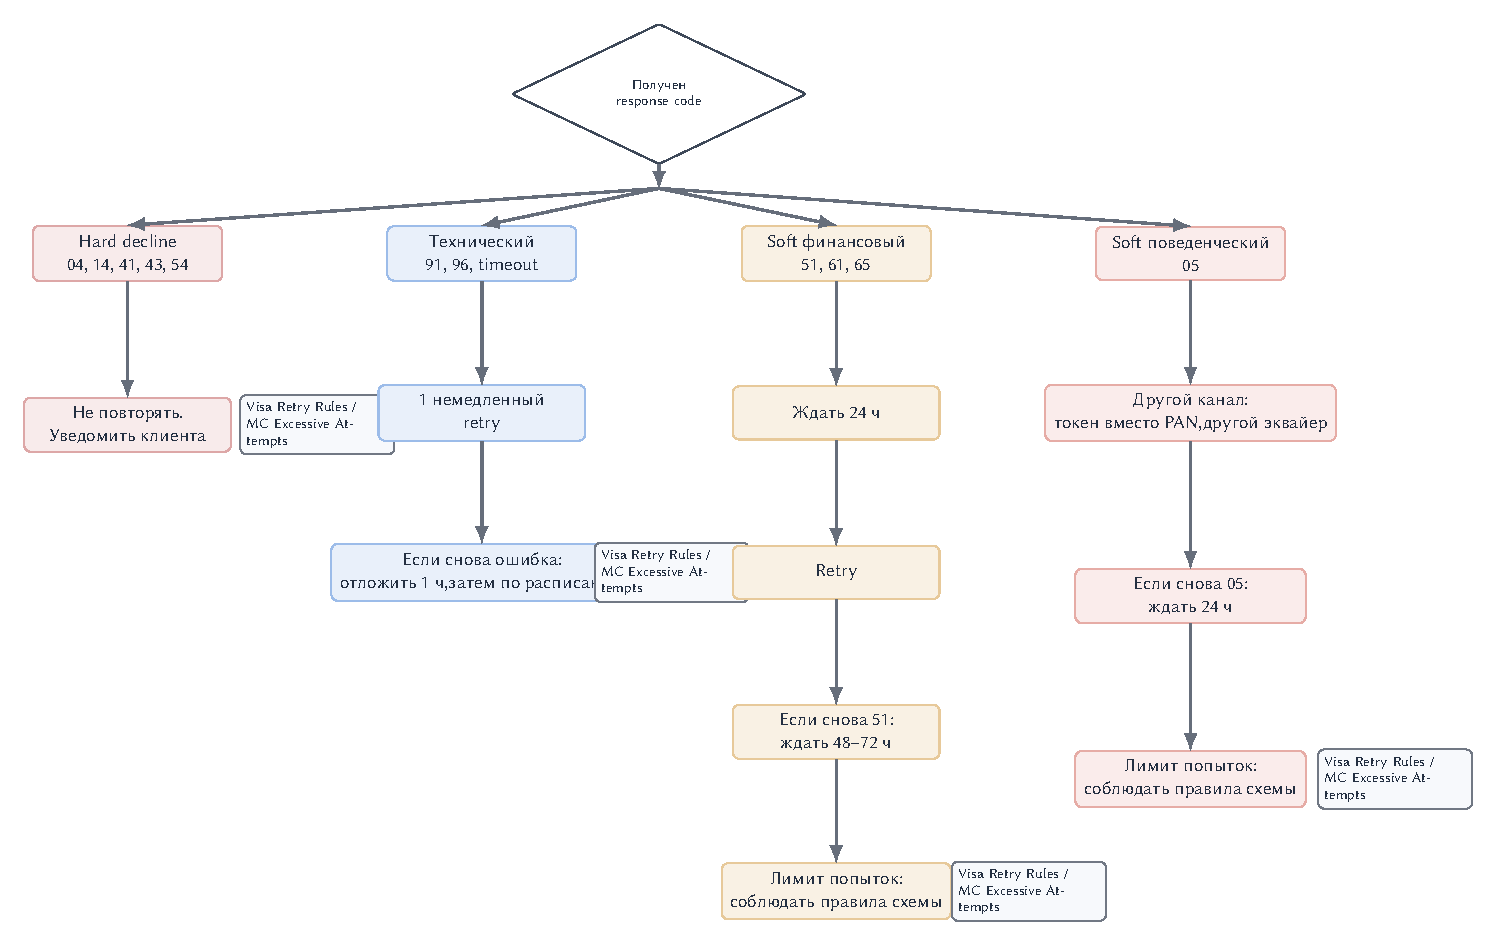
\includegraphics[width=\linewidth]{assets/figures/ch24-decline-management/decline-retry-tree.pdf}
  \caption{Логика повторов после отказа в авторизации.}
  \label{fig:decline-retry-tree}
\end{figure}

Хорошая логика повторов уменьшает не число отказов вообще, а число
бессмысленных повторных попыток. Это разные задачи, и смешивать их
опасно.

\section{Сетевой токен и PAN: дополнительный контекст доверия}
\label{sec:decline-tokens}

Представим одну и ту же подписку в двух вариантах. В первом мерчант
отправляет авторизацию с PAN, во втором --- с сетевым токеном
(network token) из Visa Token Service или MDES. Для эмитента это не
одно и то же сообщение: во втором случае он получает не только
реквизиты, но и дополнительные признаки доверия --- криптограмму
(cryptogram), уровень доверия токена (Token Assurance Level, TAL) и
привязку к домену мерчанта \sidecite{visa-vts}\sidecite{mc-mdes}.

Именно поэтому одна и та же операция при работе с PAN может выглядеть
для эмитента менее прозрачной, а при токене --- более ожидаемой. Он
видит не только номер карты, но и то, что запрос прошёл через
инфраструктуру схемы и пришёл из ожидаемого домена. Но из этого не
следует, что токен снимает все риски. Если антифрод или риск-профиль
мерчанта остаются проблемными, токен сам по себе не спасает. Его
практическая ценность скромнее и важнее: он даёт эмитенту более
богатый контекст для решения.

Есть и более прозаическая выгода: при перевыпуске карты мерчант реже
теряет контакт с реквизитом. Когда эмитент меняет PAN или дату
истечения, схема может прозрачно обновить соответствие токена новой
карте. Это уменьшает долю \rc{54} Expired Card, сокращает отток в
подписках и снижает зависимость от пакетных обновлений реквизитов.

Почему переходят не все? Причины обычно скучны и потому устойчивы.
Нужны интеграция и сертификация; если текущий поток кое-как держится,
миграцию откладывают до заметной боли в виде доли отказов и оттока;
наконец, многие мерчанты вообще не управляют токенами напрямую и
зависят от того, как быстро двигается их PSP. Поэтому разговор о
токенах почти всегда упирается не только в безопасность, но и в
операционную зрелость.

Подробнее об архитектуре сетевых токенов~--- в главе \ref{ch:tokenization}.

\section{Маршрутизация через эквайера как инструмент конверсии}
\label{sec:decline-routing}

Две операции с одной и той же картой и на одну и ту же сумму могут
закончиться по-разному только потому, что пришли к эмитенту разными
путями. Поэтому маршрутизация через эквайера влияет на долю одобрений
не меньше, чем многие изменения на стороне платёжной формы.

Во-первых, существует BIN-аффинность. Для одних BIN-диапазонов
исторически лучше работает один эквайер, для других --- другой.
Причина может быть технической, поведенческой или просто исторической:
эмитент привык видеть конкретный маршрут. На практике такую аффинность
измеряют на собственной статистике, сравнивая пары
\enquote{BIN --- эквайер}.

Во-вторых, работает каскадная маршрутизация (cascade routing). Сначала
запрос идёт через основного эквайера; если получен мягкий отказ,
система может сделать вторую попытку через резервного. Резервный
эквайер нередко имеет иной путь до эмитента и иной профиль доверия.
Прирост редко бывает драматическим, но на больших объёмах он становится
заметным \sidecite{visa-core-rules}.

Но у маршрутизации есть граница легитимности. Она не должна быть
способом обойти interchange. Если транзакцию намеренно уводят через
другую юрисдикцию ради более низкой ставки, это уже нарушение правил
схем \sidecite{visa-core-rules}\sidecite{mc-rules}. Легитимная цель
маршрутизации --- повысить долю одобрений и сократить задержку, а не
перестроить структуру сборов.

На практике всё это собирается в интеллектуальную маршрутизацию
(smart routing): движок смотрит на BIN, историю работы эквайера,
стоимость и вероятность успеха и выбирает лучший путь для каждой
транзакции. Именно поэтому крупные PSP и оркестраторы так часто
выигрывают у прямого подключения к одному эквайеру.

\section{Доля одобрений по вертикалям}
\label{sec:decline-benchmarks}

С долей одобрений всегда одна и та же ловушка: число легко назвать и
трудно понять. 85\% --- это хорошо или тревожно? Ответ зависит от
вертикали, географии, типа карты и самой модели оплаты.

Сначала надо договориться о знаменателе. Если включить в него все
авторизационные попытки вместе с техническими тайм-аутами и мусорными
запросами, получится одна цифра. Если считать только те попытки, на
которые эмитент действительно вернул код ответа, получится другая.
Именно во втором смысле ориентиры обычно и публикуют \scheme{Visa} и
\scheme{Mastercard}.

Но сами диапазоны стареют быстрее, чем успевает выйти книга. Они
зависят от вертикали, страны, доли 3DS, качества токенизации, текущих
волн мошенничества и даже календарного окна. Поэтому для печатной
главы важнее понять, как читать эти цифры, чем пытаться запомнить
конкретные проценты.

Розницу сравнивают отдельно от сервисов путешествий и перевозок,
подписки --- отдельно от разовых интернет-платежей, а MCC повышенного
риска --- отдельно от обычной розницы. Внутренний рынок почти всегда
выглядит лучше трансграничного. В подписках MIT-транзакции тоже легко
выглядят слабее, если не оформлен корректный контекст согласия: без
цепочки по правилам SCF эмитент видит обычный CNP-запрос и не видит
продолжения уже данного согласия
\sidecite{visa-scf}\sidecite{mc-scf}.

\begin{kaobox}[title=Важно, colback=red!5, colbacktitle=red!20]
  Актуальные диапазоны по вертикалям, странам и типам интеграции быстро
  меняются и не должны жить в книге как отдельная справка. Для печатной
  части важен метод: долю одобрений нужно читать только в разрезах.
  Одно число \enquote{по всему продукту} почти всегда скрывает реальные
  причины отказов.
\end{kaobox}

\begin{kaobox}[title=На практике]
  Измеряйте долю одобрений раздельно по сегментам: новые и вернувшиеся
  клиенты, карты с 3DS и без неё, PAN и токен, внутренний рынок и
  трансграничные операции. Агрегированная метрика почти бесполезна для
  оптимизации. Сегментация быстро показывает, где сосредоточены
  отказы: как правило, основную массу проблем даёт не весь поток, а
  сравнительно узкий класс транзакций с особыми характеристиками.
\end{kaobox}

\begin{chaptersummary}
\begin{itemize}
  \item Мягкий отказ (soft decline) допускает повторную попытку,
        жёсткий (hard decline) --- нет; технические коды \rc{91} и \rc{96}
        обычно оправдывают один быстрый повтор, после которого нужен
        уже разбор причины.
  \item \rc{05} Do Not Honor не объясняет причину отказа: за ним могут
        стоять антифрод, лимиты, поведенческий профиль или внутренняя
        политика эмитента; \rc{51} и \rc{54} тоже нельзя читать буквально.
  \item Visa Transaction Retry Rules and Excessive Attempt Restrictions
        и Mastercard Excessive Attempts Rules ограничивают число повторов;
        превышение допустимого числа попыток может привести к
        мониторингу.
  \item Сетевой токен (network token) даёт эмитенту более богатый контекст,
        уменьшает зависимость от перевыпуска карты и часто проходит лучше PAN,
        но не отменяет антифрод.
  \item Маршрутизация через эквайера, каскадная и интеллектуальная
        маршрутизация меняют долю одобрений и задержку, но не должны
        служить обходом interchange-правил.
  \item Долю одобрений имеет смысл читать только в разрезе сегментов:
        вертикаль, тип карты, наличие 3DS, PAN или токен, внутренний
        рынок или трансграничный поток; актуальные диапазоны нужно брать
        из свежей статистики и первоисточников рынка, а не из книги.
\end{itemize}
\end{chaptersummary}
